\documentclass[a4paper]{article}
\usepackage[utf8]{inputenc}
\usepackage{amsmath}
\usepackage{amssymb}
\usepackage{caption}
\usepackage{mathtools}
\usepackage{amsfonts}
\usepackage{lastpage}
\usepackage{tikz}
\usepackage{float}
\usepackage{placeins}
\usepackage{textcomp}
\usetikzlibrary{patterns}
\usepackage{pdfpages}
\usepackage{gauss}
\usepackage{fancyvrb}
\usepackage[table]{colortbl}
\usepackage{fancyhdr}
\usepackage{graphicx}
\usepackage[margin=2.5 cm]{geometry}

\definecolor{listinggray}{gray}{0.9}
\usepackage{listings}
\lstset{
	language=,
	literate=
		{æ}{{\ae}}1
		{ø}{{\o}}1
		{å}{{\aa}}1
		{Æ}{{\AE}}1
		{Ø}{{\O}}1
		{Å}{{\AA}}1,
	backgroundcolor=\color{listinggray},
	tabsize=3,
	rulecolor=,
	basicstyle=\scriptsize,
	upquote=true,
	aboveskip={0.2\baselineskip},
	columns=fixed,
	showstringspaces=false,
	extendedchars=true,
	breaklines=true,
	prebreak =\raisebox{0ex}[0ex][0ex]{\ensuremath{\hookleftarrow}},
	frame=single,
	showtabs=false,
	showspaces=false,
	showlines=true,
	showstringspaces=false,
	identifierstyle=\ttfamily,
	keywordstyle=\color[rgb]{0,0,1},
	commentstyle=\color[rgb]{0.133,0.545,0.133},
	stringstyle=\color[rgb]{0.627,0.126,0.941},
  moredelim=**[is][\color{blue}]{@}{@},
}

\lstdefinestyle{base}{
  emptylines=1,
  breaklines=true,
  basicstyle=\ttfamily\color{black},
}

\pagestyle{fancy}
\def\checkmark{\tikz\fill[scale=0.4](0,.35) -- (.25,0) -- (1,.7) -- (.25,.15) -- cycle;}
\newcommand*\circled[1]{\tikz[baseline=(char.base)]{
            \node[shape=circle,draw,inner sep=2pt] (char) {#1};}}
\newcommand*\squared[1]{%
  \tikz[baseline=(R.base)]\node[draw,rectangle,inner sep=0.5pt](R) {#1};\!}
\newcommand{\comment}[1]{%
  \text{\phantom{(#1)}} \tag{#1}}
\newcommand{\pd}[2]{%
  \frac{\partial^{#2}}{\partial #1^{#2}}}
\def\el{[\![}
\def\er{]\!]}
\def\dpip{|\!|}
\def\MeanN{\frac{1}{N}\sum^N_{n=1}}
\cfoot{Page \thepage\ of \pageref{LastPage}}
\DeclareGraphicsExtensions{.pdf,.png,.jpg}
\author{Nikolaj Dybdahl Rathcke (rfq695) \\
        Victor Petren Bach Hansen (grn762) \\
        Tobias Hallundbæk Petersen (xtv657) }
\title{Signal and Image Processing \\ Assignment 7}
\lhead{SIP}
\rhead{Assignment 7}

\begin{document}
\maketitle

\section*{Question 1}
\subsection*{a)}
In Figure \ref{fig:q1a} below, the dilation operation for the 3 masks can be seen, applied on a cropped picture of \texttt{text.png} (included in the image toolbox). The green pixels represent pixelvalues that are 0 after the dilation and the purple pixels represent pixelvalues that are 1 after the dilation.
\begin{figure}[H]
\begin{center}
  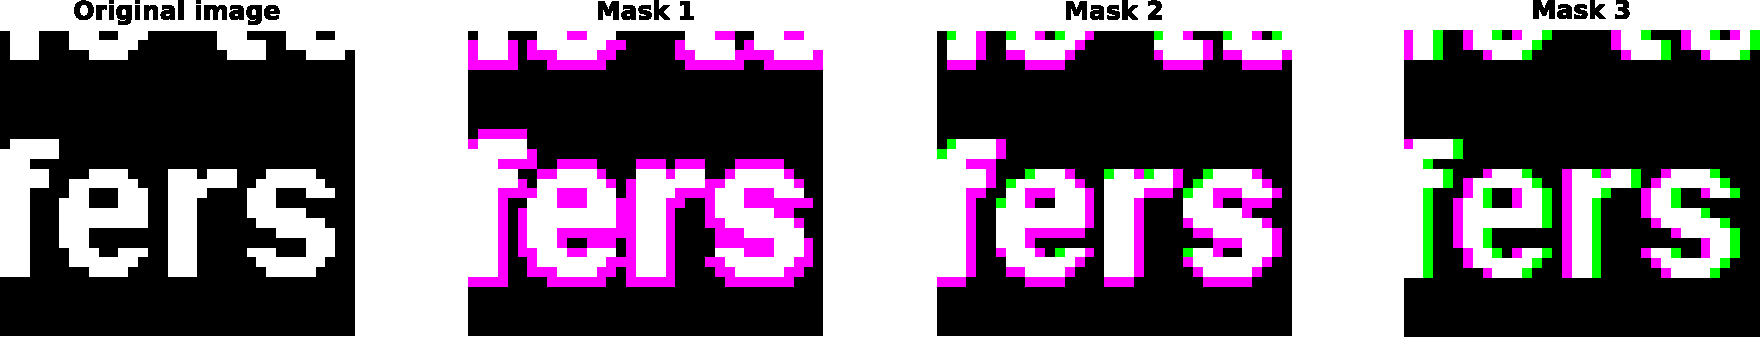
\includegraphics[scale=0.5]{q1a-crop.pdf}
\end{center}
\caption{Dilation of an image using the 3 different masks}
\label{fig:q1a}
\end{figure}
\begin{itemize}
\item We can see that the structural element used in the dilation, does not need to be symmetrical in order for it to work, but it has an effect. Since the MATLAB function \texttt{imdilate} uses a reflection of the structural element, the resulting image will not be the same as described in SB p. 200, but can be achieved by rotating the SE 180 degrees and feeding it to \texttt{imdilate}. The difference can be seen below in Figure \ref{fig:symdif}, where the rightmost picture is where the SE is
rotated (giving the result as expected from the definition in SB, since it cancels out the reflection done by MATLAB) and the middle picture is when the SE is given raw to \texttt{imdilate}:
\begin{figure}[H]
\begin{center}
  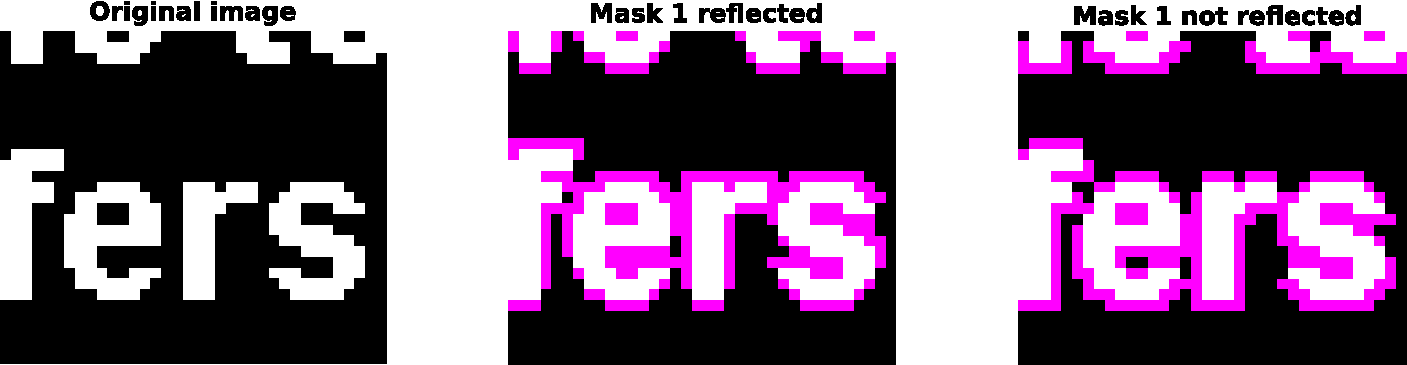
\includegraphics[scale=0.5]{q1aa.pdf}
\end{center}
\caption{Dilation of an image with an asymmetric SE. Figure shows the difference between rotating (or reflecting) and not rotating the SE.}
\label{fig:symdif}
\end{figure}

\item Figure \ref{fig:q1a} (middle right picture) also shows that there is no need for the structural element to have an odd number of pixels in both directions, as the centre pixel will be chosen to be the one north, north-west or west of the geometric centre (or in MATLAB code \texttt{floor((size(nhood) + 1)/2)}, where \texttt{nhood} is the SE), if the height or width of the mask is odd.

\item From Figure \ref{fig:q1a} we can also observe that the center pixel does not need to be set, illustrated in the rightmost picture, but since the centre pixel is not set, it will result in a shift of the image.
\end{itemize}

\subsection*{b)}
Figure \ref{fig:q1b} below shows the dilation of the masks by the image \texttt{four.bmp}.
\begin{figure}[H]
\begin{center}
  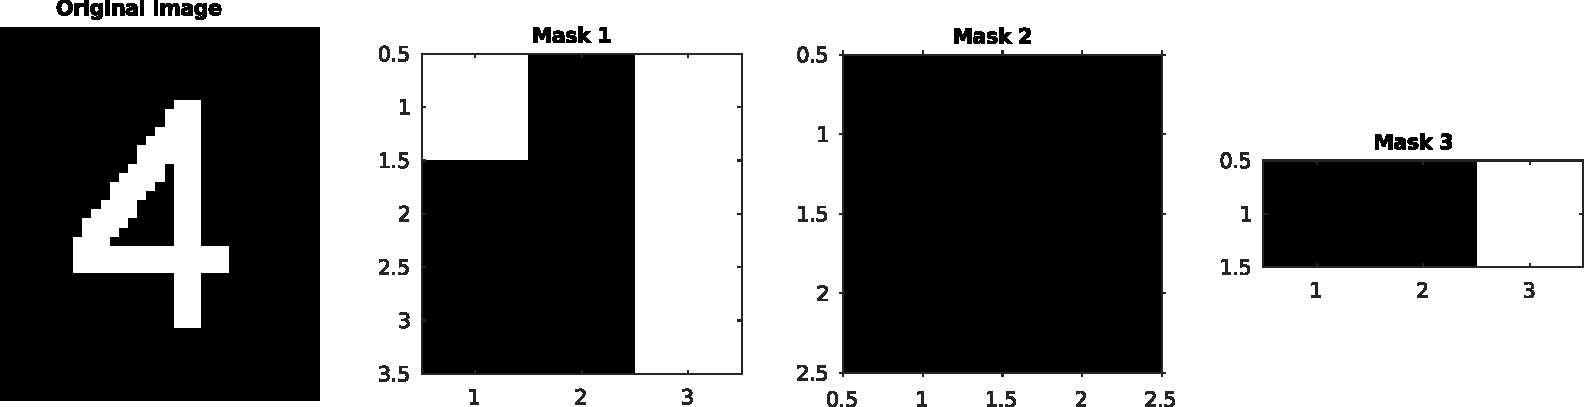
\includegraphics[scale=0.5]{q1b.pdf}
\end{center}
\caption{}
\label{fig:q1b}
\end{figure}
We can observe that the size of the image is reduced down to the size of the corresponding mask it was dilated by, which is due to MATLAB cropping the image. What the images essentially shows, is the dilation of the image by the masks, then cropped down to the size of the mask, viewed from the centre of the dilated image.
\subsection*{c)}
Figure \ref{fig:q1c} below shows the full dilation of the masks by the image \texttt{four.bmp}.
\begin{figure}[H]
\begin{center}
  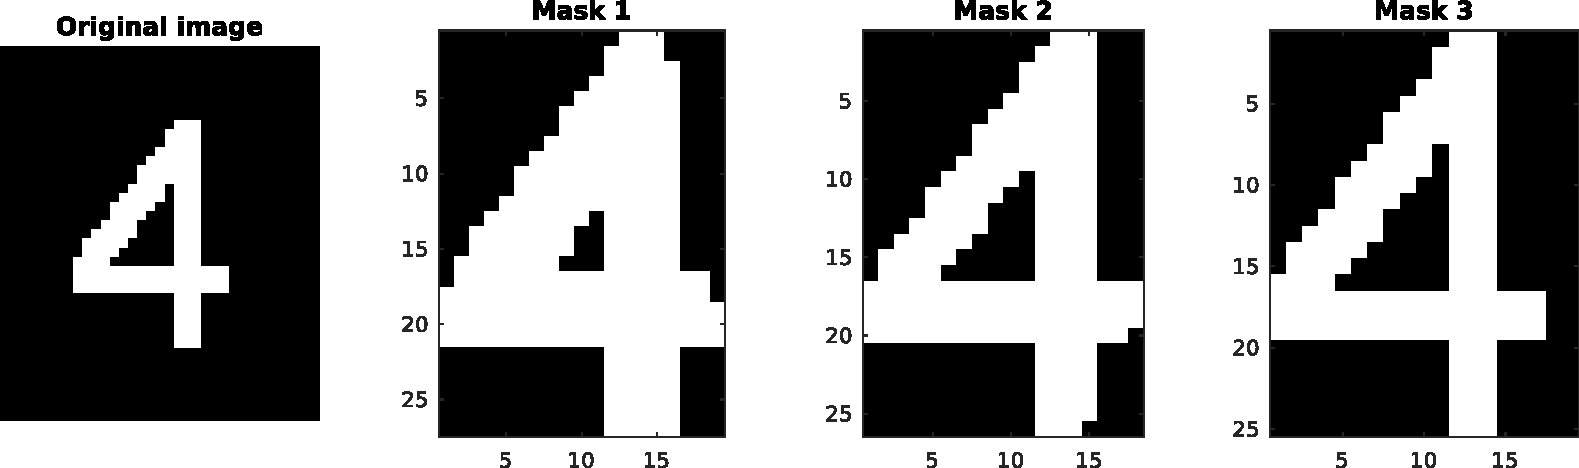
\includegraphics[scale=0.5]{q1c.pdf}
\end{center}
\caption{}
\label{fig:q1c}
\end{figure}
The images show that the full dilation of the masks by the image produces the same dilation of the image by the masks, but in a cropped version, where the surrounding background pixels have been removed by MATLAB. The full dilation of the masks by the image does not preserve the original image size, as it otherwise would the other way around.
\subsection*{d)}
As the two dilations produces the same dilated result of the foreground pixels, but in a cropped version, the SE and image can be interchangeable if we know exactly how the image was cropped, such that we are able to restore it to the full size.
\subsection*{e)}
The advantage of dilating the SE by the image, is that we have to consider alot fewer pixels, as the size of the SE often is much smaller than the image. This results in alot fewer operations when performing the (full) dilation.
\section*{Question 2}
\subsection*{a)}
Remember that opening in mathematical morphology is the dilation of the erosion of an image. The closing operation is the opposite, that is, erosion of the dilation of an image. Using Matlab's built-in function \texttt{imopen} and \texttt{imclose}, we get the resulting images from using these operation on the image \texttt{TestImageQn2.mat} seen in Figure \ref{2_1a}. Note that Matlab actually rotates the SE by $180$ degrees when performing dilation, but since the SE we use is symmetric, the result is the same.
\begin{figure}[H]
  \centering
  \captionsetup{justification=centering}
  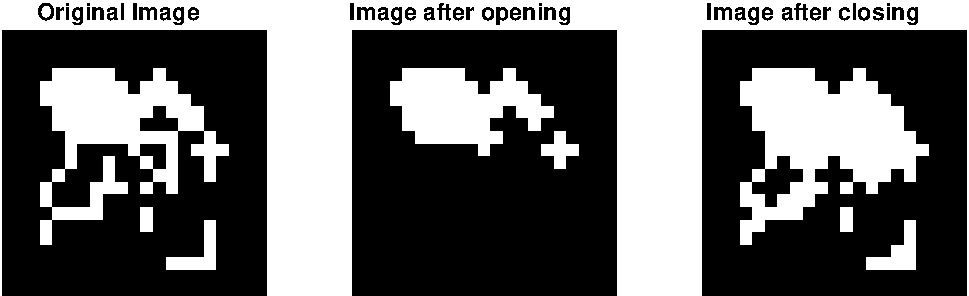
\includegraphics[width=\textwidth]{q2_1-crop.pdf}
  \caption{Figure showing the results of performing opening and closing of the image found in 'TestImageQn2.mat' with a $3$ by $3$ diamond-shaped structuring element.}
  \label{2_1a}
\end{figure}
Intuitively it makes sense that an image contains more $1$'s (in a binary image) after closing compared to after opening. When we erode an image, we remove all the set (set to $1$) pixels that do not contain the structuring element. So there are less pixels the can be dilated. But when we dilate an image first and then erode it with the same SE, we will always have the pixels from the original image. For instance, let us look at the lower left part of the image, which contains no 'plus'. When we erode this part, the entire part is removed so there is nothing to dilate on. However, if we dilated it first with some SE, we know that this SE will exist in that part, so when we erode it is not empty. The lower right corner, where there is a mirrored L-shape is another good explanation of this as it is isolated. It does not contain the SE we are using (the plus), so the entire shape is removed during the erode part of opening, which means there is nothing to dilate on. But we can see that in closing, we actually 'gain' another pixel while the original shape is also present.

\subsection*{b)}
As discussed in (a), closing will lead to more set pixels while opening will remove set pixels. One can see the the opening operation as an operation that removes small 'blobs' in an image, while the closing operation will close gaps between blobs, but still maintain blobs that are not close to other blobs.

\subsection*{c)}
To have a single blob left, the size of the SE depends on what operation we are using. If we are using opening, we can see this as removing all of the blobs but the largest one. The size of the blobs are kinda defined by how many of the SE we use that can fit in them. So we want an SE that is large enough to remove all the 'islands', which can be estimated to be the size of the next largest island. \\
If we perform closing, we sort of want to do the opposite. We want to remove the largest gap between two blobs. So having an SE that is larger than the largest gap will close the gap, and as it is the largest, it will also close all other gaps, but it will usually be enough to have a smaller SE than this. An estimation is around half the size of the largest gap (as they close the gap from both sides). A quick experiment with a $5$ by $5$ diamond as SE yields the image in Figure \ref{2_1c}.
\begin{figure}[H]
  \centering
  \captionsetup{justification=centering}
  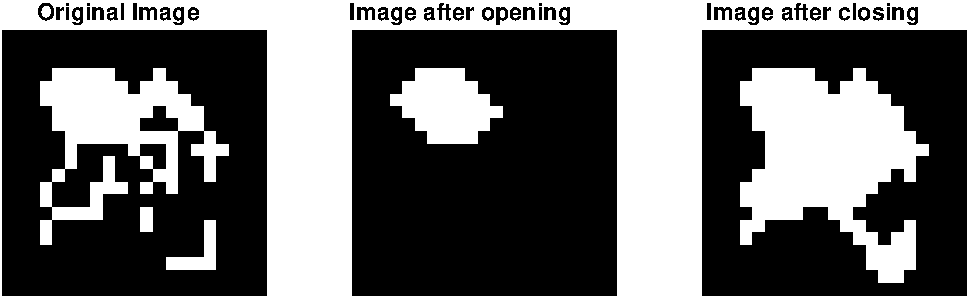
\includegraphics[width=\textwidth]{q2_1b-crop.pdf}
  \caption{Figure showing the results of performing opening and closing of the image found in 'TestImageQn2.mat' with a $5$ by $5$ diamond-shaped structuring element.}
  \label{2_1c}
\end{figure}
Which shows that it is enough to have a single resultant blob. It might be enough with a $4$ by $4$ SE, but we were not sure how to make it 'diamond-shaped'.

\section*{Question 3}
\subsection*{a)}
The hit-or-miss operation is similar to ones we used for dilation and erosion. However, when we had a $0$ in the SE, it meant that it could be whatever. We only needed to have a match where we had ones. For hit-or-miss, we want an exact match, so where there are zeroes in the SE, we must also have zeroes in the actual image to have a hit. Note that we are also able to leave fields blank (in some way), which means it is a wildcard. \\
The top-hat operation is the result from subtracting the opening of an image with a structuring element from the image itself. \\
Likewise, the bottom-hat operation is the result of subtracting the closing of an image from the image.

\subsection*{b)}
Hit-or-miss is useful when we want to find particular features. Matlab's \texttt{bwhitmiss} performs the operation given two SE's. The first one indicates what pixels must be set, the second one indicates what pixels must not be. That way, it is possible to leave "blanks" by setting that particular pixel to $0$ in both of them. Figure \ref{3a} show the results of using the function to highlight different features.
\begin{figure}[H]
  \centering
  \captionsetup{justification=centering}
  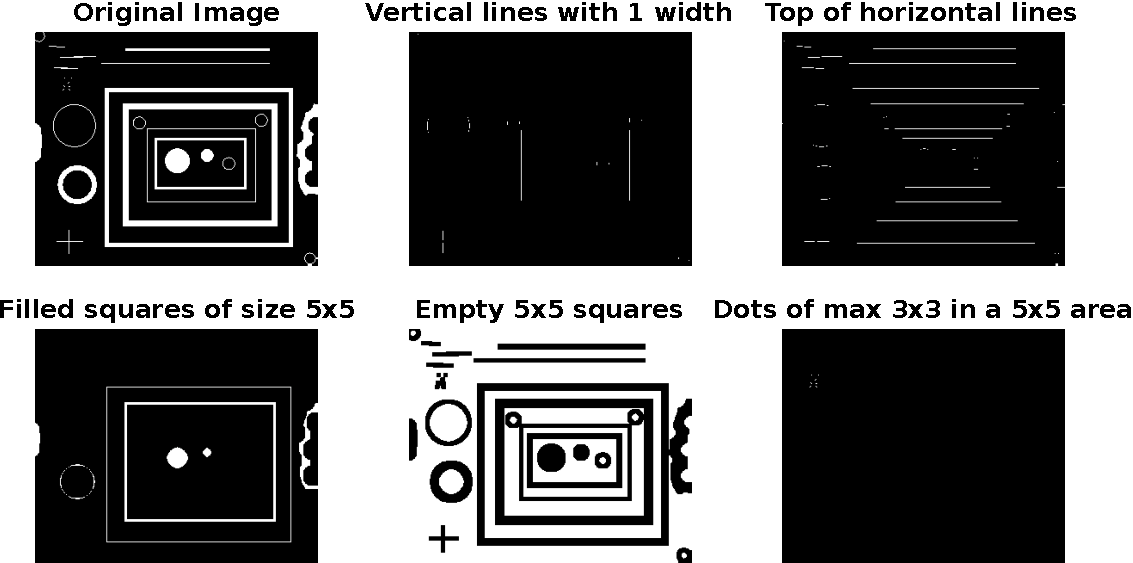
\includegraphics[width=\textwidth]{q3a-crop.pdf}
  \caption{Figure showing the result of using the hit-or-miss operation on the image \texttt{blobs.png} which highlights different features of the image.}
  \label{3a}
\end{figure}
The top images uses a $3$ by $3$ SE, while the bottom ones use a $5$ by $5$. We can see the operation is useful to find these specific features and we are able to find many special ones as we are allowed to leave blanks (such as the dots in the last image). \\
The top-hat operation is useful to find bright elements in the image that are smaller than the SE. The larger the SE is, the more elements are extracted from the image as they will fit in the SE. Figure \ref{3b} shows the results of the top-hat operation with different size and shaped SE's, namely the shapes 'diamond' and 'disk'.
\begin{figure}[H]
  \centering
  \captionsetup{justification=centering}
  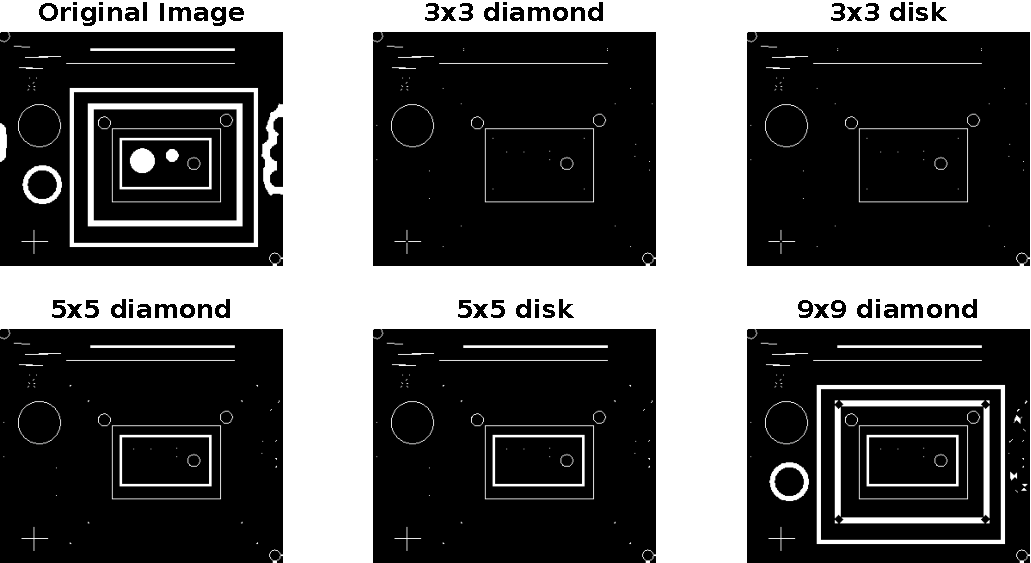
\includegraphics[width=\textwidth]{q3b-crop.pdf}
  \caption{Figure showing the result of using the top-hat operation on the image \texttt{blobs.png} which return the image that highlights bright elements that are smaller than the structuring element.}
  \label{3b}
\end{figure}
As we expected, more elements are visible as we increase the size of the SE. However, there does not seem to be much difference in the shape we use for the SE - at least not for disk and diamond. If we used a single dot in the middle though, the entire thing would be black, so the shape does makes a difference for the resulting image, but since disk and diamond are shapes that resemble each other a lot, it is hard to notice the difference. \\
The bottom-hat operation is useful for detecting dark areas in the image that are smaller than the SE. Like the top-hat, the larger the SE is, the more of these elements are visible. Figure \ref{3c} demonstrates this.
\begin{figure}[H]
  \centering
  \captionsetup{justification=centering}
  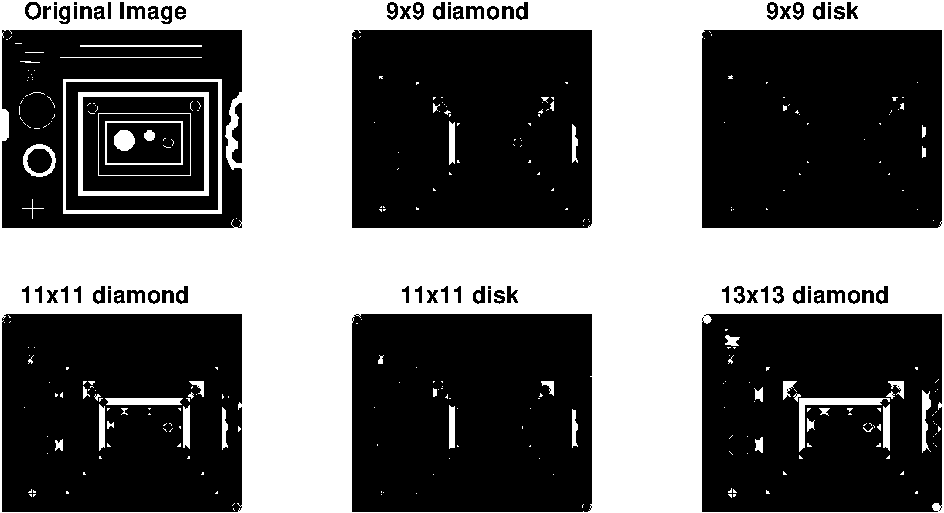
\includegraphics[width=\textwidth]{q3c-crop.pdf}
  \caption{Figure showing the result of using the bottom-hat operation on the image \texttt{blobs.png} which return the image that highlights dark elements that are smaller than the structuring element.}
  \label{3c}
\end{figure}
Again, more elements are extracted the larger the SE is, though the sizes of the SE'sare a little larger. There is a difference between the two shapes. The diamond seem to pick up more shapes than the disk, which is because the diamond is "smaller" than the disk so it will pick up the filled elements in image faster than the disk.

\section*{Question 4}
In order to correct the uneven illumination in the background of the image \texttt{rice.png}, the top-hat transformation was used, which is the difference between the image and the image after being opened (in this case with a disk SE). Figure \ref{fig:q4} below shows this operation for a number of different disk sizes.
\begin{figure}[H]
  \begin{center}
    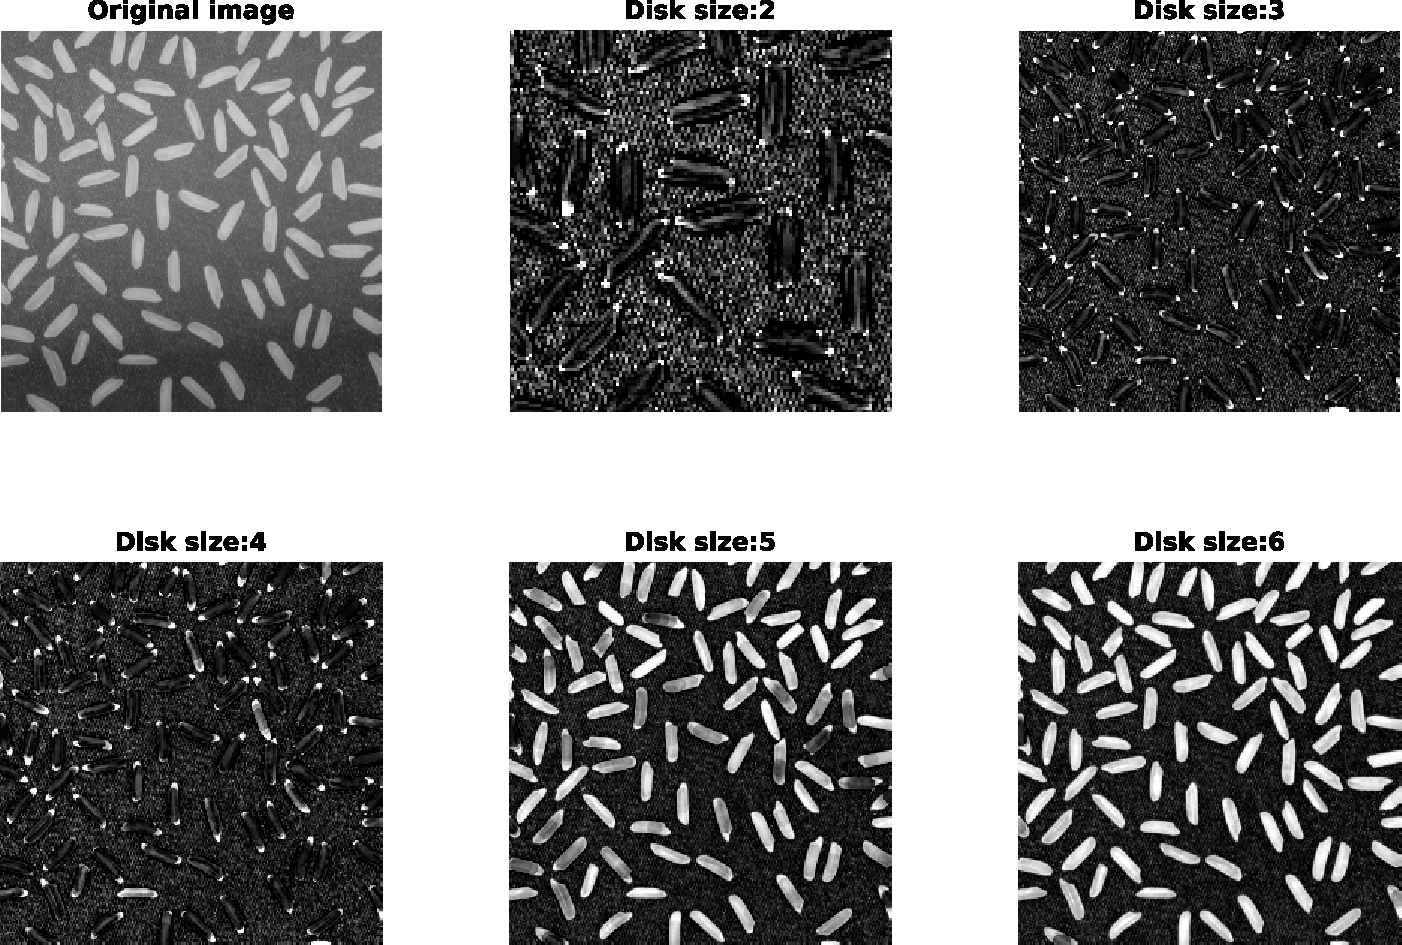
\includegraphics[width=\textwidth]{q4.pdf}
  \end{center}
  \caption{Top-hat transform of an image for various disk SE sizes.}
  \label{fig:q4}
\end{figure}
We can see from the figure, that the smallest disk radius required for isolating the background with reference to the features, is $5$ pixels. This is because of the fact that the illumination correction of the top-hat transform only works if the disk size is greater than the features we want to preserve (the rice grains), but small enough to still fit in between them. This indicates that the width of a rice grain is about $10$ pixels.

\section*{Question 5}
If we try to perform hit-or-miss with the image \texttt{five.bmp} as SE on the image \texttt{test\_digits.bmp}, we would need to have an exact match. We use the Matlab function \texttt{bwhitmiss} and try to match on both the foreground pixels and the background pixels. Doing this gives the result found in Figure \ref{5a}.
\begin{figure}[H]
  \centering
  \captionsetup{justification=centering}
  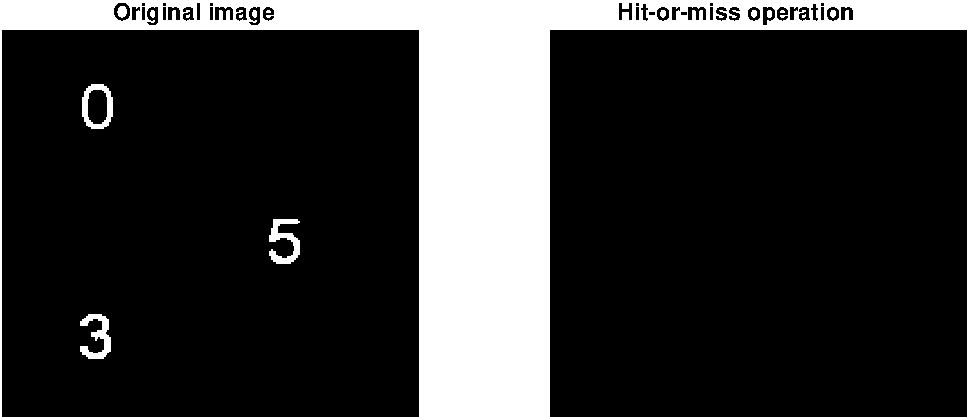
\includegraphics[width=\textwidth]{q5a-crop.pdf}
  \caption{Attempt to perform the hit-or-miss operation on the image \texttt{test\_digits.bmp} with the image \texttt{five.bmp} as the structuring element.}
  \label{5a}
\end{figure}
We can see there are not matches. This is probably because we need to match on all $41x35$ pixels, which is very strict. So we need to relax the constraints for hit-or-miss. This is done by introducing the wildcard pixels.

\section*{Question 6}
We want to make a processing pipeline to automatically extract the in focus areas of the image \texttt{flowers.jpg}, shown in Figure \ref{fig:flowers}.
\begin{figure}[H]
  \centering
  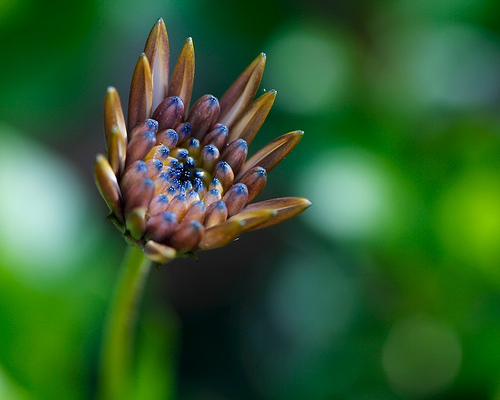
\includegraphics[width=0.6\textwidth]{./src/flowers.jpg}
  \caption{The handed out image \texttt{flowers.jpg}.}
  \label{fig:flowers}
\end{figure}
Our process is divided in to 8 steps:
\begin{enumerate}
  \item The image is converted to grayscale, this is done as we lose no 'sharpness' by grayscaling the image, and we reduce the size to work on by a factor three.
  \item A new image is then generated by blurring the image with Gaussian blur, this is subtracted from the original image, this removes many already blurry features, but retains sharp edges.
  \item We then perform edge detection by subtracting an eroded image from a dilated image, where dilution and erosion was done with a diamond SE of size 1.
  \item The image is then dilated with a diamond of size two, and eroded with a disk of size 2, this enhances some of the features of the in focus part.
  \item We then apply a threshold to the image filtering all pixels with value smaller than 5 out, and set the remaining pixels to one, which results in a mask.
  \item The outlying 'islands' are then removed by opening the mask with a diamond SE of size 3.
  \item To fill out the gaps in the mask we want to apply, we first dialate, then close and erode the image.
  \item The mask is then applied as the alpha channel to the original image, resulting in an image only showing the in focus part of the image.
\end{enumerate}
The result of each of these steps are shown in Figure \ref{fig:q6}, with the final masked image being the last of the steps.
\begin{figure}[H]
  \centering
  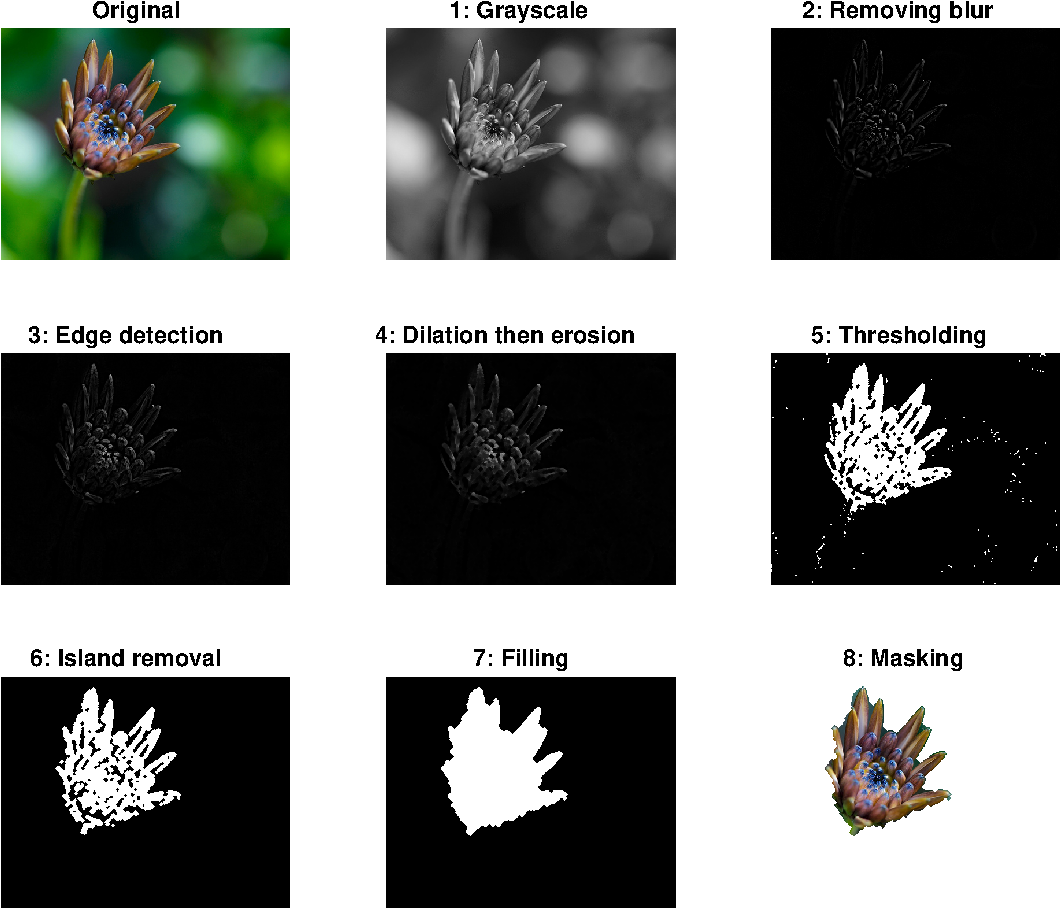
\includegraphics[width=\textwidth]{q6-crop.pdf}
  \caption{Steps to find and mask the in focus part of the image \texttt{flowers.jpg}.}
  \label{fig:q6}
\end{figure}
\end{document}
